\documentclass[../../main.tex]{subfiles}

%-----------------------------------------------------------%
\begin{document}
\chapter{Simulations \& Results}
\thispagestyle{fancy}


%-----------------------------------------------------------%
\section{Mechanical}
\blindtext
%----------------------------END----------------------------%

%-----------------------------------------------------------%
\section{Instrumentation}
\subsection{Optical Simulations}
Considering our tight requirements on the quality of image we require to analyse the system using certain parameters such as spot size which may not be available on the datasheet of a commercial lens.
Moreover considering getting our system to be custom manufactured rather than buying off the shelf, we can go for a custom made lens system for which designing is done on simulation softwares.

So, simulations provide with the results to decide on the lens system.
Zemax Optic Studio provides all the necessary tools for our purpose with sequential ray tracing.

The parameters described in section \hyperref[sec:imagespec]{8.2.1} are to be achieved in simulations for a lens system to be useful.
\newpage
Following are results for a single lens system:
\begin{align*}
    \\Focal\:length\:=&\:36mm
    \\Aperture\:=&\:15mm
    \\Total\:system\:length\:=&\:43.9mm
    \\Working\:f\#\:=&\:2.3
    \\Spot\:radius\:=&\:20\mu m\:at\:70\%\:energy 
    \\Wavelength\:considered\:for\:simulations\::&550nm
    \\Material\::&\:Fused\:Silica\:(one\:of\:the\:lowest\:temperature\:coefficients)
    \\Lens\:coating\::&\:MgF2\:(550nm)
\end{align*}
\begin{figure}[h!]
    \centering
    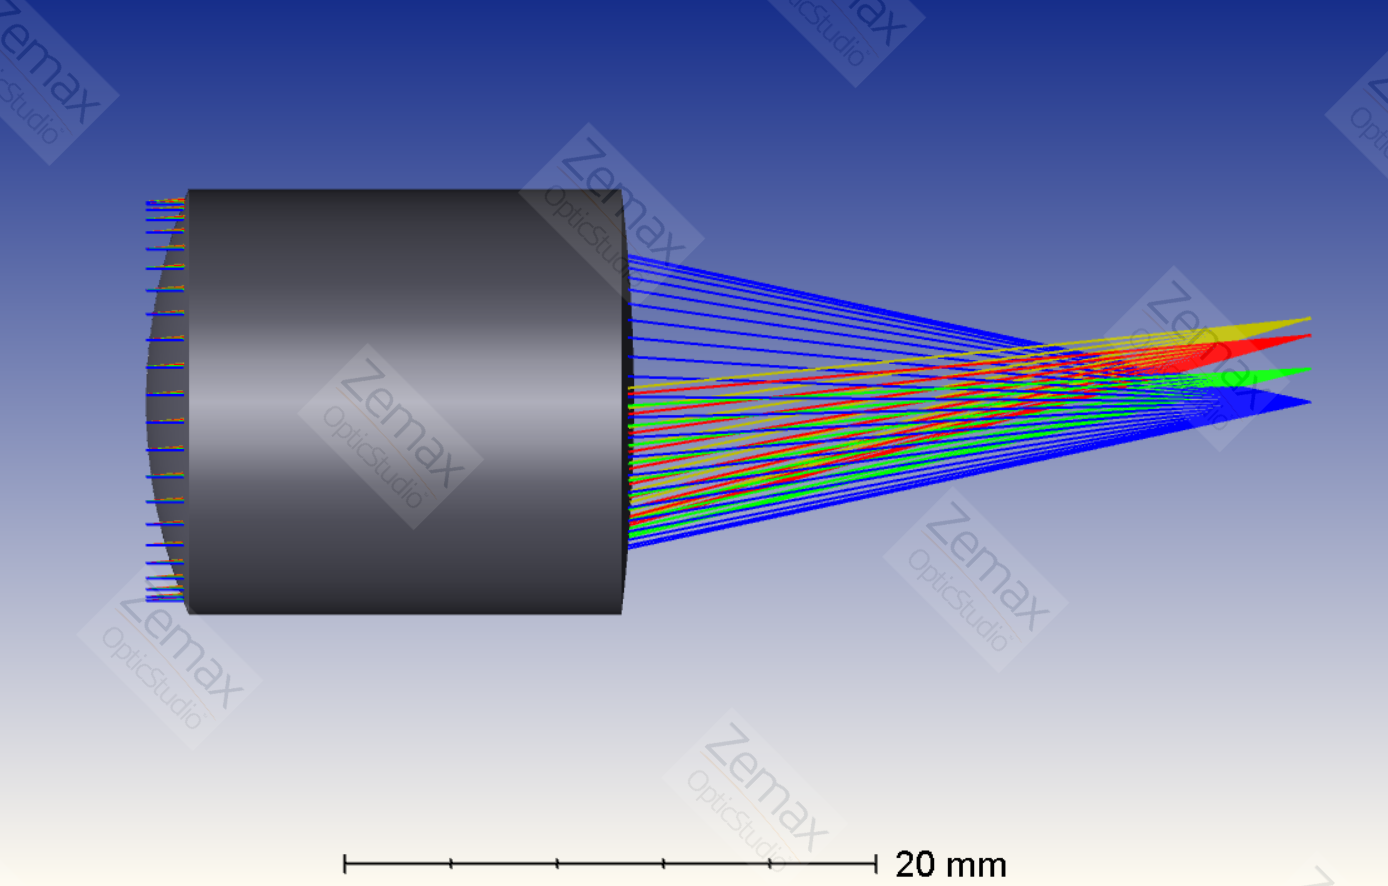
\includegraphics[width=0.5\linewidth]{Figures/Instrumentation/single_lens_3d_1.PNG}
    \caption{Solid Lens Diagram with scale :\\The different coloured lines represent light rays at different angles of incidence in FOV with blue at 0$^{\circ}$}
    \label{fig:single_lens_3d_1}
\end{figure}
\begin{figure}[h!]
    \centering
    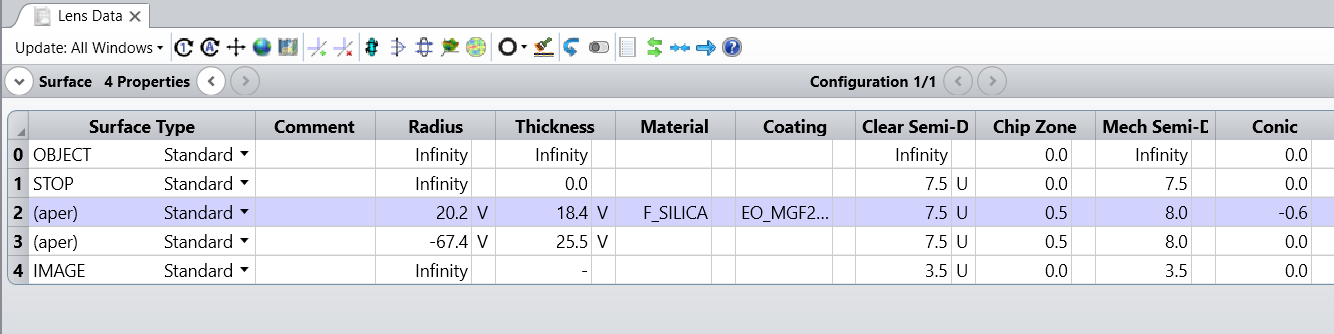
\includegraphics[width=\linewidth]{Figures/Instrumentation/single_lens_datasheet_1.PNG}
    \caption{Lens datasheet}
    \label{fig:single_lens_datasheet_1}
\end{figure}
\pagebreak[4]
\begin{figure}[h!]
    \centering
    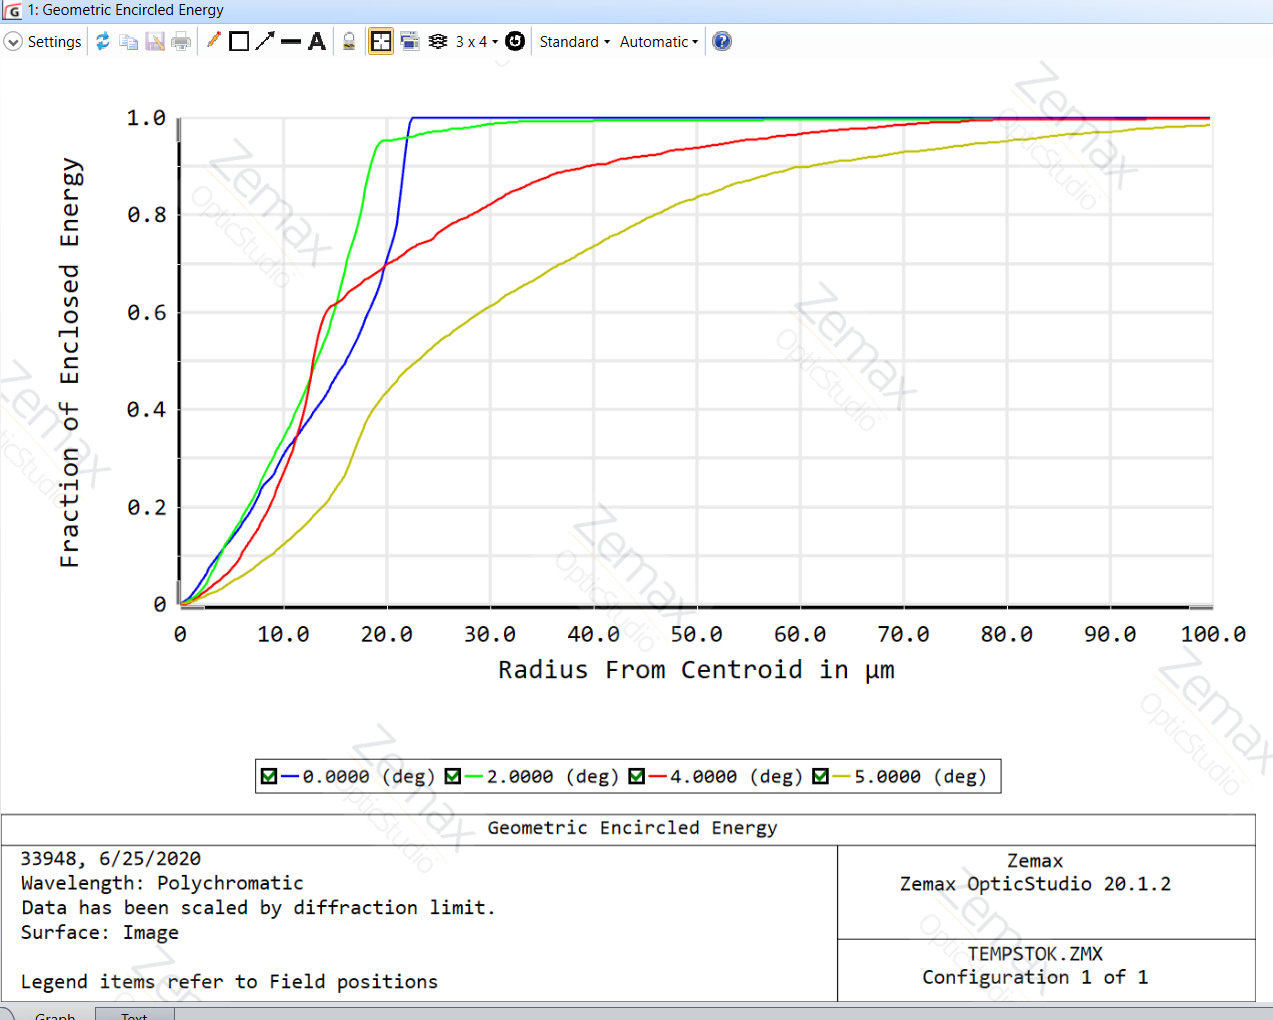
\includegraphics[width=0.75\linewidth]{Figures/Instrumentation/single_lens_spot_radius_1.PNG}
    \caption{Enclosed energy plotted against radius from centroid}
    \label{fig:single_lens_spot_radius_1}
\end{figure}
\begin{figure}[H]
    \centering
    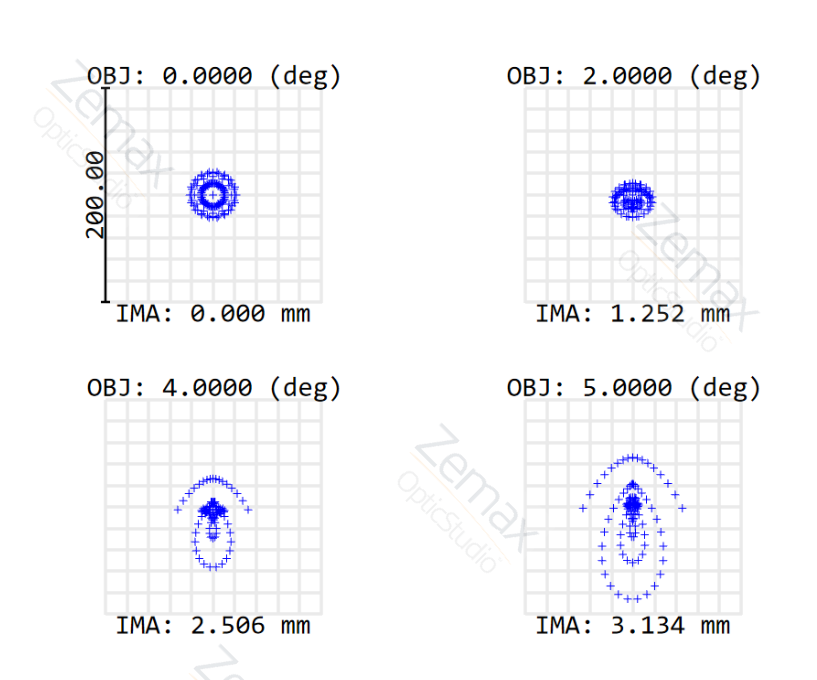
\includegraphics[width=0.75\linewidth]{Figures/Instrumentation/single_lens_spot_diagram_1.PNG}
    \caption{Spot diagram at different field points (grid is 200$\mu m\times$200$\mu m$) }
    \label{fig:single_lens_spot_diagram_1}
\end{figure}
\paragraph{NOTE:}
The spot diagram appears to distort to a great extent at 4$^{\circ}$. This is common to occur for any lens system, however it can be dealt if the weighted centroid comes to be at the same point as for a perfect image.

Multiple simulations have been done and this is one design which has been documented. Multiple lens systems have also been simulated but the results weren't satisfactory.
\subsection{Baffle Efficiency}
In order to evaluate the baffle for stray light analysis the best method is to measure the point source transmittance (PST) at the detector location. PST is defined as the ratio of stray light irradiance in the desired location at different angles relative to the optical axis at the entrance aperture of the optical system.
\vspace{1em}
\begin{center}
    $PST(\theta,\phi) =\frac{H_{d}(\theta,\phi)}{H_{c}(\theta,\phi)} $
\end{center}
\par
where, $H_d$ is the irradiance at the collecting aperture of the optical system at radial and polar angles $\theta$ and $\phi$ from the optical axis  and $H_d$ is the irradiance at the detector of the system.
\par
The following figure illustrates how a baffle with vanes works better than  a baffle with no vanes.

\par
\begin{figure}[h]
    \centering
    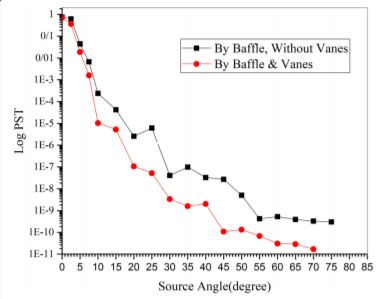
\includegraphics{Figures/Instrumentation/point_source_transmittance.JPG}
    \caption{log PST as a function of source angle}
    \label{fig:12.1}
\end{figure}

\subsubsection{Stray light analysis}
For the purpose of analysing stray light in the baffle, it has been decided to make use of the OpticStudio software by Zemax.

\par
The OpticStudio GUI provides an option of non-sequential ray tracing which allows importing standard STEP files or SolidWorks Parts and Assemblies. With the help of correctly placed detectors, it is possible to determine the effectiveness of the baffle.

\begin{figure}[H]
    \centering
    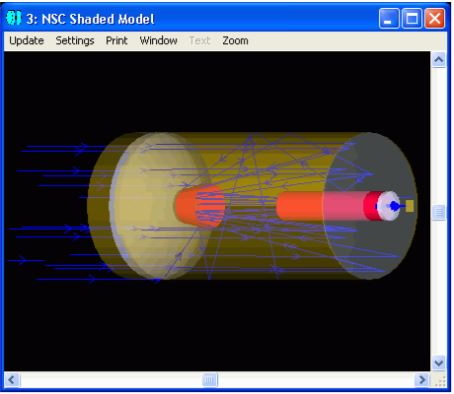
\includegraphics{Figures/Instrumentation/non_sequential_component.JPG}
    \caption{Non-sequential ray tracing in Zemax OpticStudio}
    \label{fig:12.6} 
\end{figure}
\par
\textbf{\underline{Note:}} There have been no simulations performed for the baffle as the software is still being explored.

%----------------------------END----------------------------%

%-----------------------------------------------------------%
\section{Model-in-Loop Simulation}
\blindtext
%----------------------------END----------------------------%
\end{document}